\documentclass{rapport}
\usepackage{lmodern,textcomp}
\usepackage{lipsum}
\usepackage{float}
\title{Rapport Stage Antoine POSNIC M1} %Titre du fichier

\begin{document}

%----------- Informations du rapport ---------

\titre{Consultant Centre de Contact (CTI)} %Titre du fichier .pdf
\UE{Rapport de stage} %Nom de la UE
\sujet{Du 04/03/2019 au 30/08/2019} %Nom du sujet

\eleves{Antoine \textsc{POSNIC}} %Nom des élèves

\enseignant{Gilles \textsc{LESVENTES}\\
        	Ophélie \textsc{GAUTIER}} %Nom de l'enseignant


%----------- Initialisation -------------------

\fairemarges %Afficher les marges
\fairepagedegarde %Créer la page de garde
\afterpage{\null\newpage}
\tabledematieres %Créer la table de matières

%------------ Preface----------------
\section*{Remerciements}
Avant toute chose, je tiens à remercier l'équipe pédagogique du Master 2 Ingénierie Logicielle pour la formation qui m'a été donnée, ainsi que le moyen d'effectuer ce stage.\\
Je remercie bien évidemment l'équipe des Ressources Humaines de Capgemini Rennes, qui m'a aidé et fait confiance pour mon retour dans l'entreprise après mon stage de Master 1.\\
Je remercie Ophélie GAUTIER et son équipe, pour m'avoir accepté et accueilli dans ce projet, ainsi que les différents membres du cluster* Centres de contact (CTI) de Capgemini Rennes.\\
Ils m'ont permis de m'intégrer rapidement dans le groupe, de progresser et ont répondu à toutes mes interrogations.\\
Finalement, je tiens à remercier Olivier BARAIS, pour le partage des informations de rédaction pour ce rapport.

\newpage
\section*{Preface}
Cette préface a pour but d'introduire mon stage ainsi que l'entreprise. Je commencerai par annoncer le contexte dans lequel j'ai effectué mon stage, le sujet et les objectifs de ce dernier, ainsi qu'un bref descriptif de l'entreprise. Enfin, je finirai sur le plan du rapport.

\subsection*{Contexte}

Pour valider ma fin de deuxième année de Master Ingénierie Logicielle, j'ai effectué un stage chez Capgemini, une ESN (Entreprise de Services du Numérique) s'imposant à l'international. Ce stage de six mois s'est déroulé du 4 mars au 30 août 2019. Il a eu lieu sur le site de Rennes, au sein de la people unit CSD (Custom Software Development).
Lors de ma recherche de stage, plusieurs entreprises se sont montrées ouvertes à ma candidature. Mais Capgemini a finalement réussi à me convaincre notamment grâce à mon expérience précédente passée chez eux lors de mon stage de Master 1.
\\

Mon but était d'expérimenter davantage la vie en entreprise en intégrant à part entière une équipe, tout en continuant à découvrir de nouvelles technologies non-traitées lors de mes cinq années en université.
\\
Mes demandes pour accepter le stage se résumaient en deux points primordiaux.
Je voulais, dans un premier temps, participer entièrement à la vie du projet que j'allais rejoindre, et non pas répondre à un sujet pour stagiaires cherchant à expérimenter des solutions qui pourraient "peut-être" bénéficier à un réel projet dans le futur. Je voulais participer et expérimenter le vrai travail d'un développeur au sein d'une véritable équipe.
Ensuite tout comme l'année précédente, j'ai demandé d'être assigné à un projet sur des technologies que je n'avais pour le moment pas touché. L'année précédente, il s'agissait du C++ couplé au framework Qt, et cette année il me restait encore le C\# avec le framework .NET sur ma liste de technologies à découvrir.\\
Sous l'écoute de mes exigences, les équipes de ressources humaines de Capgemini m'ont rapidement orienté vers un sujet de stage spécifique. Comme il s'agit d'une grande entreprise, les projets acceptant des stagiaires étaient nombreux. Cependant, une grande majorité de ces projets étaient orientés Java/JEE, mais je voulais quelque chose de nouveau.\\

Ainsi, je me suis vu attitrer un projet, comme désiré, en C\#/.NET avec la mission de consultant pour les centres de contact du grand groupe d'assurrance français. Ce projet existe chez Capgemini depuis près de 10 ans après avoir été repris d'une ESN concurrente, pour maintenir et faire évoluer les besoins de leurs solutions de centres de contact. Avec ce thème de stage, j'étais motivé pour participer aux actions de l'équipe sur ce projet, où je découvrirais de nouvelles technologies.

\subsection*{Annonce du plan}

Ce rapport a pour but de présenter le déroulement de mon stage chez Capgemini. Il vient donc de bon sens de commencer par présenter cette dernière, son rôle à l'international et ses avantages.
Un chapitre sera dédié à la définition et l'explication d'un centre de contact.\\
J'expliquerai ensuite en quoi consiste le projet Pacifica, agrémenté de points techniques sur son fonctionnement.
Ensuite, j'aborderai le cadre dans lequel j'ai effectué mon stage, l'équipe avec laquelle j'ai travaillé ainsi que son organisation.\\
Et pour finir, la dernière partie traitera de mes activités effectuées durant le stage.

\newpage
%------------ Corps du rapport ----------------

%---------------- Chapter 1 -------------------
\section{Capgemini}

Je vais présenter ici l'entreprise Capgemini, dans un premier temps dans sa globalité, pour ensuite me concentrer sur l’activité Rennaise et du grand Ouest. Je retracerai son histoire, son marché, ses activités et les avantages qu'elle peut fournir à ses collaborateurs.

\subsection{A l'international}

A l'origine française et créée par Serge Kampf en 1967, Capgemini est aujourd'hui un leader mondial dans l'industrie du conseil et des services informatiques. Anciennement nommée Sogeti (Société pour la Gestion de l'Entreprise et le Traitement de l'Information), c'est en acquérant Gemini Computer Systems en 1974 et CAP en 1975 qu'elle s'approche de son nom actuel avec : Cap Gemini Sogeti. Mais ce ne sera qu'à partir de 2004 que le groupe a changé son nom pour l'actuel «Capgemini».\\

Leur politique d'acquisition les pousse après plus de 50 ans d'existence à détenir un total de plus de 30 entreprises autour du globe, spécialisées dans le secteur des nouvelles technologies. On notera notamment le rachat cet été d'Altran.
Estimée à plus de 16 milliards, Capgemini compte environ 200 000 employés et possède près de 10 000 collaborateurs en France ainsi qu'un important pôle de sous-traitance en Inde. Le reste s’étale dans plus de 40 pays différents, ce qui peut offrir des opportunités à l'international.

\subsection{Activité}

Capgemini étant une ESN, elle s'appuie sur trois principaux pôles de métiers : le domaine du conseil, des services informatiques et de l'infogérance.
\begin{itemize}
  \item \textbf{Conseil ou Consulting Services (CS):} consiste à diriger ses clients dans les transformations que ces derniers veulent accomplir, que ce soit pour améliorer leur croissance ou leur compétitivité. On parle par exemple ici de transformation digitale.
  
  \item \textbf{Services Informatiques ou Technology Services (TS):} ce pôle conçoit et développe des systèmes demandés par les clients.
  
  \item \textbf{Infogérance ou Outsourcing Services(OS):} il permet l'accompagnement d'un client partiellement ou intégralement pour un de ses systèmes. 
\end{itemize}
\vspace{5mm}
Ces trois pôles donnent à Capgemini un réseau important de clients à travers différents secteurs.

\begin{itemize}
  \item Le secteur publique, avec des clients comme la DGA, ainsi que des administrations telles que le ministère de la Défense.
  
  \item Les services financiers, assurances ou banques comme dans le cadre de mon stage.
  
  \item Le secteur du commerce et du transport, fournissant par exemple une plate-forme de e-commerce pour la SNCF.
  
  \item Les Télécoms, Médias et divertissements, comme  Orange, SFR, Bouygues, M6 et Canal+ actuellement clients chez Capgemini Rennes.
  
  \item Énergies, Utilities et Chimie.
  
  \item Industrie, Automobile et Sciences de la vie.
\end{itemize}

\subsection{Capgemini Rennes}

Le site Capgemini Rennes se situe depuis 2015 sur la ZAC des Champs-Blancs à Cesson-Sévigné, au sein de la pépinière Digital Square. Elle est entourée d'entreprises du secteur digital. \\

On y retrouve deux principaux groupes nommés people units : les CSD (Custom Software Development), plus orientés vers la conception de nouveaux systèmes, et les AMS (Application Developpement Maintenance), pour la maintenance et les évolutions de systèmes déjà délivrés chez le client. En plus, on retrouve une petite partie de DCX (Digital Customer Experience) pour les travaux de consulting, ainsi qu'une équipe de RH et RM (Ressource Manager).\\

Plus de 1100 collaborateurs sont présents sur ce site, pour une moyenne d'âge de 35 ans. Il y a une constante évolution puisque les équipes de recrutements visent environ deux cent nouveaux recrutements chaque année. 

\subsection{Avantages}
Un tel grand groupe dispose de nombreux avantages.\\

Capgemini Rennes dispose premièrement d'un CE, ayant plus de cinquante salariés. Il offre un lieu de vie où des jeux de société et livres sont à disposition, ainsi que divers avantages et réductions pour les employés (ex : réductions pour des activités culturelles et sportives, des chèques-cadeaux, des réductions pour des billets de Cinéma / Spectacles / Sport / Loisirs...)\\

On y retrouve aussi des syndicats, permettant de protéger et/ou informer les employés de la structure des nouvelles mesures mises en place par la direction, ainsi que des inégalités dont ils pourraient être victime. Lors de mon stage,  différents flyers de syndicats ont été partagés, informant notamment d'une nouvelle mesure comme par exemple la mise en place d'accords d'intéressements.\\

Capgemini offre des tickets restaurant de 8,60€ payés à 60\% par l'employeur (soit le maximum possible dans la loi Française), une mutuelle, un régime de prévoyance santé, ainsi qu'une complémentaire retraite ou PERCO.\\

Pour les congés, un salarié commence à 25 jours par an en ajoutant une nouvelle journée en fonction de l'ancienneté. On trouve aussi de 8 à 10 RTT par an.\\

Un point important est aussi mis sur les formations. Gros plus pour un développeur, puisqu'il doit pouvoir s'adapter et se mettre à jour dans cet environnement grandissant qu'est l'informatique, restant au goût du jour tout le long de sa carrière. De plus, les certifications qui en découlent sont reconnues dans le monde du travail par le poids que Capgemini a sur le marché.\\

De plus, cette ESN conseille fortement l'utilisation des communautés, qui permettent notamment l'échange d'informations entre ses différents acteurs d'un corps de métier. Par exemple la communauté d'ingénieurs "software engineer" propose des présentations techniques de divers technologies/frameworks.

Les formations et communautés permettent aux collaborateurs de ne pas rester cloisonnés dans un seul type d'activité, offrant la possibilité à terme d'apprendre et changer de corps de métier.\\

En effet, comme on peut voir sur la figure ci-dessous, on a ici la possibilité de diverger vers de nouveaux types de métiers, sous les conseils de son carrière Manager (un supérieur avec qui le collaborateur peut partager ses désirs d'orientation de carrière au sein du groupe).\\

\insererfigure{fig/fig1_ChoixCarriere.png}{7cm}{Choix de carrières.}{Carriere}

Enfin, comme il s'agit d'une ESN touchant à un large horizon de projets, les RM affirment être disponibles pour assurer une possible migration vers d'autres projets. 

\subsection*{Conclusion}

Capgemini est une grande entreprise réputée dans le monde du Digital. Sa taille offre une diversité non-négligeable de projets, la qualifiant ainsi souvent d'une entreprise initiatique pour de nouveaux arrivants dans le monde du numérique.
Elle offre de nombreux avantages, et promet une flexibilité dans le plan de carrière de ses collaborateurs.

\newpage

%---------------- Chapter 2 -------------------
\section{Centres de contact}

Lors de ce stage, j'ai travaillé autour des solutions pour un centre de contact. Il devient donc important dans un premier temps d'expliquer ce qu'est un centre de contact, ainsi que de définir les tenants et aboutissants d'une telle infrastructure.\\
Ainsi, dans une première partie, nous allons décrire le travail d'un centre de contact ainsi que les rôles qu'il peut jouer pour une entreprise.\\
Ensuite, nous allons parler de l'organisation de ces centres de contact, de leur fonctionnement, et des diverses solutions digitales disponibles pour la coordination de ces derniers.\\
Je finirai enfin avec un exemple concret autour de la solution utilisée dans le cadre de mon projet.

\subsection{Définition et rôles d'un centre de contact}

Un centre de contact peut être visualisé comme une interface entre une entreprise et ses clients. Il offre divers services pour ces derniers ; que ce soit fournir des informations, prendre des rendez-vous ou encore offrir une assistance.\\

Il joue ainsi un rôle primordial dans l'entretien de la clientèle de l'entreprise, offrant des services parfois primordiaux.
Les actions d'un centre de contact peuvent être larges, et varient énormément selon l'activité de l'entreprise qu'elles servent.\\

Par exemple :\\
Un centre de contact d'un grand groupe d'assurance fournira une assistance administrative dans le cadre d'un sinistre, délivrera des attestations de couverture sociale (par exemple), ou encore offrira des moyens de modifier son contrat d'assurance.\\
Tandis qu'un centre de contact destiné à un grand revendeur mondial s'occupera plutôt de Services Après Vente (SAV) et de la gestion de commandes.
De part leur nature, ces centres se veulent faciles d'accès pour leurs clients. C'est pourquoi ils offrent généralement de nombreuses techniques pour les interroger (mails, téléphone, chat-boxes, etc...). Cela pose donc des soucis de coordination et d'orchestration des données.
C'est ce que nous allons traiter dans cette seconde partie.

\subsection{La technique derrière un centre de contact}

Le terme centre de contact défini une activité industrialisée du contact client. Il s'agit alors d'un secteur à part entière d'une entreprise, avec ses propres systèmes et techniques.
D'un point de vue structurel, les centres de contact à l'échelle industrielle restent généralement les mêmes.\\

Ils se composent de divers centres de services clients, où sont employés des opérateurs formés à répondre à certains types de problématiques dont les clients ont besoin. Ainsi, chaque demande doit être analysée pour être dirigée vers un opérateur compétent, et pour cela, il existe diverses solutions logicielles.\\

Chacune possédant leurs propres spécifications, ces solutions cherchent à répondre aux différents besoins métiers de leurs clients.
On retrouve par exemple des techniques pour constamment améliorer la satisfaction client, ou un système de monitoring afin d'évaluer les performances du service. On peut aussi retrouver une planification horaire pour concilier les périodes de pointe et emploi du temps des opérateurs.\\

Ces solutions logiciels sont nombreuses. On retrouve par exemple :
Avaya ; Genesys ; Cisco ; Odigo ,...
Dans le cadre de mon stage, c'est la solution Genesys qui est implémentée afin d'offrir des applications d'administration et d'interaction avec son noyau.

\subsection{La solution Genesys}

Développée par l'entreprise du même nom, Genesys est un concentré de solutions pour l'orchestration de centres de contact. Il offre des fonctionnalités de management d'opérateurs, de routages de requêtes vers des ressources adaptées, ainsi que du monitoring de performances pour l'assurance de la satisfaction client.\\

\insererfigure{fig/fig2_LogoGenesys.png}{3cm}{Logo Genesys}{Logo Genesys}

Genesys est ainsi un énorme logiciel composé d'une multitude de services et autres solutions qui peuvent, moyennant des licences, s'imbriquer entre eux.\\

On retrouve cependant comme élément principal le socle Genesys, aussi appelé Customer Interaction Management (CIM), qui est la plateforme principale pour la suite Genesys. Il fournit un environnement standard pour designer, déployer et manager en temps-réel des interactions entre clients et entreprises.
Ces interactions sont routées vers les ressources compétentes, supportant des canaux d'interactions comme de la voix, e-mails, vidéos, chat ou encore SMS, le tout selon les configurations et stratégies de l'entreprise l'utilisant.

Il offre aussi une plateforme de SDK qui expose les différents protocoles Genesys sous la forme d'une API, afin d'intégrer directement la suite à des infrastructures de centres de contact déjà existant ou d'applications personnalisées.\\

Ainsi, Genesys est une solution hautement configurable, avec de nombreux outils différents pour paramétrer ses différents composants. Pour le routage, on retrouve par exemple l'Interaction Routing Designer (IRD) qui implémente une interface nodale pour définir notamment le chemin d'une requête client.

Mais l'un des composants principaux de configuration est le Configuration Manager (CME). Ce dernier permet de paramétrer tous les objets et données dont un centre de contact à besoin, généralement sous la forme de Dossiers/Sous-Dossier. On peut y attribuer des valeurs à différents objets (par exemple une compétence spécifique à un opérateur, ou encore un métier à un site de centre de contact).

\insererfigure{fig/fig3_CME.png}{7cm}{UI du configuration Manager}{CME}

Tous ces outils de configuration permettent l'intégration de solutions de centre de contact, peu importe l'activité ou le scope de l'entreprise nécessitant ce centre.

\subsection*{Conclusion}

Les centres de contact jouent un rôle primordial dans l'activité d'une entreprise au service de particuliers. Ils permettent à la fois d'entretenir une bonne relation client avec l'entreprise, et de fournir des services qui sont nécessaires pour son bon fonctionnement.\\
Évidemment, les services et le fonctionnement d'un centre de contact varient énormément selon l'activité de la société. Selon le type d'activité ou encore la taille de cette dernière, pratiquement chacune nécessite sa propre solution selon ses problématiques.\\
Pour cela, des solutions comme Genesys permettent d'offrir des solutions industrielles, hautement configurables, autour desquelles une entreprise peut instaurer son propre système de centre de contact.

\newpage

%---------------- Chapter 3 -------------------
\section{Pacifica}

Destinée à une compagnie d'assurances aux dommages, déclarant en 2018 comme étant le premier bancassureur dommages de France, avec 12 millions de contrats sous sa tutelle et 3.77 milliards de chiffres d'affaires.\\

Pacifica répond donc aux problématiques d'un relativement grand groupe de services d'assurances pour particuliers. Nécessitant l'implémentation de centres de contact, afin d'offrir leurs services à leurs clients. Ce groupe a fait appel à Capgemini afin de concevoir et maintenir deux solutions primordiales pour le bon fonctionnement des centres de contact du groupe.

Pour commencer, je vais expliquer les problématiques globales du projet, avant de décrire plus en détail chacune des deux applications qu'il conçoit et maintient.


\subsection{Le projet Pacifica}

Le projet Pacifica développe et entretien deux applications hautement configurables : le bandeau et Ocean.\\
Ces deux projets répondent chacun à des problématiques distinctes pour un centre de contact, mais utilisent et partagent toutes deux des services et entités communes. Le tout, grâce au pro-logiciel Genesys qui leur permet à la fois de manipuler et stocker des données nécessaires pour le métier, mais aussi de configurer ces deux applications pour satisfaire leur architecture d'application hautement configurable.\\
Cela leur permet par exemple de réarranger des modules, changer de formats de données, ou encore designer leurs propres pages en fonction de divers paramètres comme le type d'utilisateur ou les types de sites. Le tout est possible sans toucher une ligne de code et en temps réel (juste rafraîchir l'application) au travers du configuration manager (CME).

Contrairement au reste du cluster Centres de contact, le projet Pacifica ne s'occupe pas de la partie Genesys. En effet, la filiale possède déjà une équipe travaillant autour de la solution, configurant leurs propres environnements pour les différents sites et opérateurs sous leur responsabilité. Ainsi, ils s'occupent de toute cette partie pouvant aller des règles de routages au management des équipes, tout en passant par les systèmes de monitoring, de configurations cisco, ou encore de manipulations des médias.\\

Ils possèdent donc de leur coté leur propre environnement Genesys, avec d'autres services et applications, qui nous sont inconnus. Mais les deux applications que nous fournissons doivent tout de même pouvoir s'y intégrer, en leur laissant aussi la possibilité d'en modifier le contenu (changer des formulaires, l'affichage des pages, cacher des fonctionnalités) selon leurs configurations.\\
Pour cela, le projet possède, pour l'environnement de développement, une panoplie de machines virtuelles sur lesquelles sont installés les différents services nécessaires, ainsi que son propre environnement Genesys parallèle à la production.

De plus, on notera que comme Genesys est utilisé en quelque sorte comme un back-end avec ses API pour en modifier le contenu, faisant tomber Pacifica comme majoritairement un projet de front-end.\\

\subsection{L'application Bandeau}

Le Bandeau Multimédia est la première application du projet Pacifica. Développée et soutenue par Capgemini depuis plus de 10 ans, le Bandeau est un client lourd destiné aux opérateurs d'un centre de contact du groupe d'assurance. Il est installé sur chaque machine et est utilisé comme outil de travail principal des agents. Il leur permet notamment, en suivant la configuration Genesys, de recevoir et traiter des requêtes clients, que ce soit:\\

\begin{itemize}
\item Répondre à des appels téléphoniques qui leur ont été désignés par le système de routage.
\item Accomplir des tâches comme la création de nouveaux contrats d'assurances ou la déclaration d'un sinistre.
\item Archiver des documents envoyés par le client en base de données, comme par exemple des attestations de résidences.
\end{itemize}

\subsubsection{Fonctionnalités}

\begin{minipage}{0.65\textwidth}
Au premier abord, on pourrait s'attendre à un tout petit logiciel. Mais de part son architecture hautement configurable, il cache en réalité un très grand nombre de fonctionnalités selon les métiers de l'agent connecté.\\

Le tout est dans un espace restreint, car le bandeau doit être ouvert continuellement sur le poste de l'agent en restant au premier plan, mais ne pas occuper trop d'espace disponible.  
\end{minipage}
\begin{minipage}{0.25\textwidth}
\insererfigure{fig/fig4_BMfront.png}{4.5cm}{Le bandeau}{BMFront}\raggedright
\end{minipage}
\vspace{10mm} %5mm vertical space
\noindent
\\

Ainsi, le bandeau est composé de cinq zones principales :

\vspace{5mm} %5mm vertical space
\begin{minipage}{0.25\textwidth}
\insererfigure{fig/fig5_BMzones.png}{10cm}{Zones du bandeau}{BandeauZones}
\end{minipage}
\begin{minipage}{0.65\textwidth}

\begin{itemize}
\item -	Zone 1 : la zone du mode \\
Cette zone permet de visualiser son mode de réception d’appel, de tâche et de mail en cours, et de le modifier.\\

\item -	Zone 2 : la zone de l’état\\
La zone 2 peut permettre de visualiser l’état global (voix et acTion), son sous-état en cours, et de les modifier. L'agent peut notamment passer dans un état "Pas libre" pour une pause déjeuner ou une réunion par exemple.\\

\item -	Zone 3 : une zone d’informations.\\
L'arrivée de messages d'information à destination de l'agent est possible grâce à cette zone, comme par exemple la notification d'une nouvelle réunion. \\

\item -	Zone 4 : Onglets\\
Cette zone contient les deux onglets voix et acTion. 
Les onglets permettent de visualiser, par un code couleur, l’état du bandeau pour chaque canal et d’accéder aux fonctions pour chaque média.
\end{itemize}

\end{minipage}
\vspace{10mm} %5mm vertical space
\noindent
\\

\vspace{5mm} %5mm vertical space
\begin{minipage}{0.65\textwidth}
Le premier onglet permet donc de recevoir, comme son nom l'indique, des appels qui ont été routés vers l'agent par Genesys. \\

Il s'agit d'un téléphone VoIP (Voice over IP) Cisco, et l'utilisateur peut à la fois répondre sur l'application ou sur son téléphone Cisco physique, appeler vers l'extérieur de l'écosystème du centre de contact, ainsi que consulter sa messagerie vocale et son journal d'appels.\\

\end{minipage}
\begin{minipage}{0.25\textwidth}
\insererfigure{fig/fig6_BMphone.png}{5cm}{Onglet Téléphone}{BMFront}
\end{minipage}
\vspace{5mm} %5mm vertical space
\noindent
\\

Le second onglet nommé "AcTion" permet de visualiser et traiter les tâches/e-mails distribués par le routage Genesys en fonction de différentes règles de gestion.\\

L'agent peut y rédiger de nouveaux e-mails, créer de nouvelles tâches, et les réaffecter à un tiers. Mais il permet surtout à l'utilisateur d'accéder aux bannettes qui sont les conteneurs principaux pour tous les médias manipulé par ce dernier. \\
Il existe de nombreux types de bannettes configurables, pouvant aller de "ma bannette" pour les tâches et e-mail de l'agent connecté, à la "Bannettes Commune", contenant des actions partagées pour tout le monde. Le tout en passant par des bannettes filtrant un type d'action comme la "Bannette E-mails"\\


\insererfigure{fig/fig7_BMetendu.png}{8cm}{Bandeau avec la bannette Emails}{BMEtendu}

Dans le cas, par exemple, où l'utilisateur sélectionne un mail dans sa bannette, il peut directement :\\
Répondre à l'e-mail, le suivre, l'imprimer, le transférer, le qualifier (associer des attributs comme l'origine, le site, ...), commenter, envoyer en Gestion Électronique de Documents (GED) afin d'archiver des pièces jointes pertinentes, identifier le contrat/client/sinistre, ou encore supprimer et clore cet e-mail.\\

Dans le cas d'une tâche, l'agent a le même type de fonctionnalités, cependant il ne lui est pas montré un corps de mail, mais plutôt un formulaire complet correspondant aux informations nécessaires pour cette tâche. Elle est configurable sur Genesys, grâce notamment au Configuration Manager (CME).

\subsubsection{Points techniques}

Le bandeau est développé en C\#, à l'aide du framework .NET 4.7 (Visual 2013 - MSBuild 12.0). Ce choix provient principalement du fait que l'écosystème des solutions chez le client tourne autour des services windows, et qu'une homogénéité était désirée (Webservices hébergés sur windows IIS, authentifications au travers des sessions windows, ...).\\
Étant un client lourd sur windows, c'est le sous-système graphique Windows Presentation Foundation (WPF) qui est utilisé, avec la librairie Telerik fournissant pour WPF une panoplie de composants graphiques supplémentaires.\\

Bien qu'ayant au fil des années subis des évolutions ici et là, dégradant l'intégrité de son patron de conception, c'est le Model-View-ViewModel (MVVM) qui est ici utilisé. La raison de ce choix est très simple: inventé par Microsoft, le patron MVVM est appliqué par WPF et Silverlight avant lui.\\

Pour les autres outils, on retrouve pour la gestion de version un repository Subversion (SVN).\\
Une plateforme de test HP Application Lifecycle Management (HP AML) pour les tests fonctionnels, et le reporting de defects par le client.\\
Enfin, pour l'environnement de compilation, un Jenkins est utilisé pour automatiser le build de livraison, tout comme lancer des builds journaliers pour s'assurer de l'intégrité du SVN après les commits de la journée.

\subsection{L'application Ocean}

Ocean est la deuxième application du projet Pacifica. Développée initialement par une ESN concurrente, elle a été reprise et soutenue par Capgemini depuis un an, suite à une refonte graphique. Ocean est un client léger destiné aux administrateurs d'un centre de contact du groupe d'assurance. Il s'agit d'une Single Web Page Application accessible par un nombre limité de personnes, offrant des outils d'administration fonctionnels et techniques. Chaque métier n'a pas accès au même type d'outils, mais dans sa globalité, ces derniers permettent notamment de:\\

\begin{itemize}
\item Configurer des utilisateurs, pour modifier leurs skills, durée de travail, ou autre.
\item Gérer des absences d'un opérateur.
\item Configurer l'écosystème Pacifica, que ce soit routage Genesys, répertoires pour le Bandeau, ou autres.
\item Consulter l'historique des modifications de paramètres.
\item Programmer des modifications.
\item Envoyer des Broadcasts sur les bandeaux.
\item Gérer des postes d'un agent (postes téléphoniques, migrations de postes de travail)
\end{itemize}

\subsubsection{Fonctionnalités}

L'application Ocean est principalement un outil centralisant et simplifiant l'administration d'objets Genesys. Tout comme le bandeau, Ocean possède une architecture hautement configurable, avec des fonctionnalités paramétrables, ou encore accessibles selon les métiers de l’agent connecté. Ainsi, le client peut modifier les labels de l'application, ranger chaque fonctionnalité dans différents groupes et les cacher en fonction des accréditations de l'utilisateur connecté.

\insererfigure{fig/fig8_OceanMain.png}{7cm}{Page d'accueil Ocean}{OceanMain}

\begin{minipage}{0.55\textwidth}

La navigation se fait au travers d'un menu déroulant configurable. Ce dernier permet d'accéder à différentes catégories, elles-mêmes supportant plusieurs fonctions. Représentées sous forme d'onglets, ces fonctions sont les éléments constituant la fonctionnalité d'Ocean, et ce sont leurs accès qui sont vérifiés en fonction des compétences de l'utilisateur. Il est donc possible que dans une catégorie regroupant six fonctionnalités, un utilisateur ne soit pas accrédité pour en observer que trois.

\end{minipage}
\begin{minipage}{0.45\textwidth}
\insererfigure{fig/fig9_OceanBurger.png}{3cm}{Menu de Navigation}{BMFront}
\end{minipage}
\vspace{5mm} %5mm vertical space
\noindent
\\

Chaque onglet contient donc une fonction indépendante de l'application, tenant sur une seule page, et qui doit correspondre à des exigences générales de l'outil. Nous pouvons citer les exemples suivants : gérer les accès concurrents à l'application et ses données critiques, paramétrer des messages et libellés de l'application, respecter les principes ergonomiques mis en place à l'initialisation du projet.\\

A ce jour, l'application Ocean comporte près de vingt-cinq fonctions techniques et/ou fonctionnelles. On peut y retrouver par exemple, rangées par catégories :

\vspace{5mm} %5mm vertical space
\begin{itemize}

\begin{minipage}{0.5\textwidth}
\item Administration Fonctionnelle
        \begin{itemize}
        \item Absences
        \item Configuration Utilisateurs
        \item Répertoires Bandeau
        \item BroadCast
        \item Réunion Plénière
        \item Visualisation Utilisateurs
        \end{itemize}
    \vspace{5mm} %5mm vertical space
    \item Matrice d'appel
        \begin{itemize}
        \item Matrices des combinatoires
        \item Restauration Matrice
        \end{itemize}
    \vspace{5mm} %5mm vertical space
    \item États Métier et Site, Scénarios
        \begin{itemize}
        \item Scénario
        \item Exceptions Métiers
        \item Etats Sites
        \item Exceptions Sites
        \end{itemize}
\end{minipage}
\begin{minipage}{0.5\textwidth}
    \item Configuration du Routage
        \begin{itemize}
        \item Départements et Zones Géographiques
        \item Entraide UGS
        \item Pourcentage Skill
        \item Zones Géographiques et UGS
        \end{itemize}
    \vspace{5mm} %5mm vertical space
    \item Administration Technique
        \begin{itemize}
        \item Création Utilisateurs
        \item Gestion Verrous
        \item Gestion Postes Téléphoniques
        \item Migration Poste de Travail
        \item Suppression Utilisateurs
        \end{itemize}
    \vspace{5mm} %5mm vertical space
    \item Programmation et Historique
        \begin{itemize}
        \item Historique
        \item Programmation
        \end{itemize}
\end{minipage}
\end{itemize}

\insererfigure{fig/fig10_OceanFonctions.png}{9cm}{Divers onglets de l'application Ocean}{OceanFonctions}

\subsubsection{Points techniques}

Ocean est développée en C\#, à l'aide du framework .NET 4.7 (Visual 2015 - MSBuild 14.0). Ce choix provenant principalement du fait que l'écosystème des solutions chez le client tourne autour des services windows, et qu'une homogénéité était désirée (Webservices hébergé sur windows IIS, authentifications au travers des sessions windows, ...).\\
Étant un client léger web, c'est le framework ASP.NET MVC (basé sur ASP.NET) qui est utilisé, avec la librairie Telerik fournissant une panoplie de composants graphiques supplémentaires.\\

En plus d'utiliser les API de l'environnement Genesys pour manipuler les paramètres ou objets de la solution, Ocean utilise d'autres services. Il implémente par exemple l'API AXL pour l'interfaçage cisco, les services de l'environnement windows pour les traitements en différé, ou encore directement un service du Bandeau pour l'envoie de broadcast aux agents d'un site.\\

Le projet a initialement été développé par une autre ESN concurrente sous le framework Silverlight aujourd'hui obsolète. Capgemini a été contractée pour créer une refonte globale de l'application, reprenant ainsi la logique des services développés par l'ESN concurrente, et recréer intégralement la partie client de l'application.\\
Pour cela, un nouveau patron de conception est utilisé: le Model-View-Controller (MVC). De plus, plusieurs couches applicatives ont été désignées dont les plus importantes sont:\\

\begin{minipage}{0.35\textwidth}
\insererfigure{fig/fig11_OceanModuleArchi.png}{3cm}{Modules}{OceanModuleArchi}
\end{minipage}
\begin{minipage}{0.55\textwidth}
La couche client comportant les modules où sont rédigées les fonctions de l'application, regroupées dans des projets C\# qui sont rangés par similarités. Par exemple, les fonctionnalités "Configuration Utilisateurs", "Visualisation Utilisateurs" et "Absences" sont toutes regroupées sous un même projet "Utilisateur".
\end{minipage}
\vspace{5mm} %5mm vertical space

\begin{minipage}{0.35\textwidth}
\insererfigure{fig/fig12_OceanWebservicesArchi.png}{3cm}{WebServices}{OceanWebservicesArchi}
\end{minipage}
\begin{minipage}{0.55\textwidth}
La couche WebService comporte à la fois la logique anciennement développée et la nouvelle, découpée dans 4 étapes. La partie "Service" qui joue le rôle d'API, représentant la façade des divers appels possibles. "Rules" où est rédigé la logique d'un appel au web service. Et enfin les couches "DAL" et "BO" appliquant les modifications au travers d'appels simples vers les API externes.
\end{minipage}
\vspace{5mm} %5mm vertical space
\\

Pour les autres outils, on retrouve un repository Subversion (SVN) pour la gestion de version.\\
Une plateforme de test HP Application Lifecycle Management (HP AML) pour les tests fonctionnels, et le reporting de defects par le client.\\
Et enfin, pour l'environnement de compilation, un Jenkins permettant d'automatiser le build de livraison, tout comme de lancer des builds journaliers pour s'assurer de l'intégrité du SVN après les commits de la journée.

\subsection*{Conclusion}

Le projet Pacifica chez Capgemini a pour but d'entretenir et faire évoluer deux applications pour une filiale d'assurance Française. Elles doivent s'intégrer et utiliser l'écosystème Genesys installé  afin de répondre aux besoins de leurs centres de contact.\\

Développé en C\# avec le framework .NET, ces deux applications peuvent être visualisées de la façon suivante:

\insererfigure{fig/fig13_PacificaApplications.png}{7cm}{Applications du projet Pacifica}{PacificaApplications}

On retrouve le bandeau, client lourd installé sur la machine de tout les opérateurs, leur fournissant les requêtes clients routées par la solution Genesys qu'ils doivent traiter. Ces dernières peuvent prendre la forme d'appels entrants ou encore d'e-mails.\\

La seconde application, nommée Ocean est un client léger web sur lequel les administrateurs d'un centre de contact peuvent manipuler une partie de paramétrage Genesys de façon sécurisée et simplifiée.

\newpage

%---------------- Chapter 4 -------------------
\section{Cadre de stage}

Je vais ici parler de l'environnement dans lequel j'ai pratiqué mon stage autour de la problématique de centre de contact.
Dans un premier temps, je parlerai de l'équipe, avec les rôles de chaque collaborateurs. Puis, je poursuivrai sur le projet, son but, son histoire, ainsi que quelques précisions techniques.

\subsection{Environnement}

Pour ce stage, j'ai donc intégré la "people unit" CSD (Custom Software Developpement). Cette dernière a pour directive principale la réalisation d'applications/solutions customisées pour ses clients.\\

Au sein de ce groupe, je me suis retrouvé dans le "cluster CTI", un open space regroupant les experts centres de contact de Capgemini Rennes. Il se constitue d'une douzaine de collaborateurs avec des profils divers, s'occupant de la réalisation et du paramétrage d'outils pour ses clients nécessitant la mise en place d'un centre de contact.\\

Dans ce cluster j'ai ainsi rejoins une petite équipe de développeurs travaillant pour un grand groupe de services d’assurances pour particuliers Français. Cette équipe, tout comme le cluster en général, a connu dans le passé un taux d'activité bien plus important, entraînant en partie une diminution drastique de ses effectifs ces derniers mois.

\subsection{L'équipe}

Constituée initialement de cinq collaborateurs, l'équipe travaillant sur Pacifica est un petit groupe comparé à d'autres existants sur le site.
On y retrouve:\\

\begin{itemize}
  \item Ophélie GAUTIER, Engagement Manager (EM) de grade C. Elle supervise et orchestre les actions de chacun sur le projet Pacifica, ainsi que d'autres projets du cluster Centre de contact (CTI). Elle est ma tutrice de stage, et elle s'est assurée de mon intégration au projet ces six dernier mois.\\
  
  \item Matthias MUSSHE, initialement responsable technique du projet Pacifica, ingénieur logiciel de grade B avant de quitter le groupe Capgemini un mois après mon arrivée. Il m'a notamment aider à comprendre et configurer le pro-logiciel Genesys, pour le bon fonctionnement de mon environnement de développement.\\
  
  \item Mohammed HAMMAMI, Ingénieur Logiciel de grade B, architecte de l'application Ocean du projet Pacifica. A encadré mes actions sur Ocean, validant mon travail comme conforme à l'architecture de cette dernière. Quittera le projet mi-juillet, ne laissant plus qu'un ingénieur sur Pacifica.\\
  
  \item Bastien CLOAREC, Ingénieur Logiciel de grade B, devenu responsable technique du projet Pacifica, il travaille notamment plus sur l'application Bandeau du projet Pacifica. Ainsi, il m'a fait découvrir l'architecture de cette application, et m'a orienté pour mes actions sur cette dernière.\\
  
\end{itemize}

\subsection{Travail en équipe}
Capgemini possède des règles pour le travail en équipe sur le site. Chaque collaborateur a le statut de cadre, cela signifie qu'il n'y a pas de comptage d'heures, juste une plage allant de 36 à 39 heures. Il existe cependant tout de même une plage horaire où la présence de chacun est attendue (9h15 -17h30).\\

Chaque matin, les équipes doivent se réunir pour un DSTUM (Daily STand Up Meeting) , une courte réunion à heure fixe (celle pour mon projet était à 9:15). Elle a pour but de se mettre à jour sur les informations générales du projet, des avancées ou retards que chaque collaborateur peuvent rencontrer, et mettre au point les actions faites le jour précédent et à venir. Cela permet d'avoir une vue globale de l'avancée du projet, ce qui semble primordial dans le cas d'un travail d'équipe.\\

Capgemini promouvoit l'utilisation de la méthode de Lean pour le développement et l'industrialisation de ses projets. Cependant, le choix de ce type de méthodes dépend du sujet et du client.\\ 
Dans notre cas, les responsables groupe d'assurance désiraient s'impliquer un minimum dans la vie de développement des évolutions qu'ils commandent. Ainsi, les méthodes agiles à la mode de nos jours n'ont pas été envisagées.\\

Ainsi, c'est le développement en V qui a été sélectionné, sur les différentes d'évolutions commandées par le client.\\


Toute évolution commence avec une Expression de Besoin (EB) rédigée par le client, suivie d'une proposition commerciale (PROPAL). Notre réponse est donnée après étude des besoins et estimation des charges de travail. Si cette évaluation du chiffrage convient au client, le projet démarre comme informé ci-dessous.

\insererfigure{fig/fig2_PhasesProjet.png}{5cm}{Cycle du projet pour une évolution.}{Cycle de vie}

Malgré le fait qu'il s'agisse d'un développement en V ou normalement le client est exclut du processus de développement. Dans le cas de ce projet, des réunions hebdomadaires sont organisées, afin faire le point sur les problèmes globaux, les timelines, ainsi que l'assurance des actions de chaque acteur du projet.

\subsection*{Conclusion}

Le projet Pacifica est considéré comme un petit projet, avec une poignée de développeurs.\\
A ses débuts, l'activité était bien plus importante avec davantage d'ingénieurs. Cependant, étant un projet en développement en V dépendant des expressions de besoins du client, il connaît des périodes d'activité réduite justifiant parfois la diminution d'effectifs.\\


\newpage

%---------------- Chapter 5 -------------------
\section{Travaux effectués}

Ce chapitre traite de mon activité lors du stage. Dans un premier temps, je vais parler du calendrier de mes actions, pour ensuite rentrer dans les détails de chacune de mes activités jugées plus importantes.

\subsection{Calendrier}

Mon stage s'est déroulé du 04/03/2019 au 30/08/2019:\\

\insererfigure{fig/fig14_Calendar.png}{6.5cm}{Calendrier d'actions lors de mon stage}{Calendar}

Il a consisté en plusieurs petites actions tout le long de ces six mois. Ce calendrier est relativement général, car il s'agit de la trame globale de mon stage, considérant le fait  que je suis revenu sur des travaux précédents après être passé à un sujet différent.\\

Par ordre catégories, je vais maintenant décrire mes tâches accomplies durant ce stage. 

\newpage
\subsection{Découverte du projet}

A mon arrivée sur le projet, je devais d'abord m'installer avec le PC qui m'a été fourni. Il s'agissait d'installer les deux environnements de développement pour le bandeau est Ocean.\\
Pour cela des documents d'installation étaient rédigées pour informer des outils et configurations nécessaires pour chaque écosystème. Bien que parfois obsolète ou obscure, Matthias a été présent pour m'aider.\\

Au terme de cette installation, je me suis retrouvé avec les outils suivant:\\

\begin{itemize}
  \item Visual Studio 2013 et 2015, les IDE (environnement de développement intégré) des projet Bandeau et Ocean respectivement. Ils supportent chacun la version MSBuild et .NET nécessaire pour leurs propre projets, avec divers plugins:
  
    \begin{itemize}
        \item AnkhSVN, pour accéder au repository distant SVN directement depuis l'IDE
  
        \item StyleCop, afin de s'assurer de l'homogénéité du code produit en appliquant des règles de syntaxe supplémentaires.
  
        \item PartCover qui lors des tests MSBuild, permet de mesurer la couverture de tests de l'application.
    \end{itemize}

  \item TortoiseSVN pour accéder au repository distant SVN indépendemment.
  
  \item Cisco IP Communicator avec PhonerLite pour simuler le téléphone d'un agent sur le bandeau.
  
  \item Genesys configuration Manager (CME)
  
  \item Ainsi que divers outils utiles du type: soapUI, Postman, mgRemote.
  
\end{itemize}

Ainsi que mon propre profil configuré genesys et cisco, pour interagir avec les deux solutions du projet comme un véritable utilisateur, avec ses propres compétences et accès paramétrables.\\

Cette période a aussi été pour moi l'occasion de découvrir l'environnement .NET que je ne connaissais pas, en parcourant les différentes documentations ou suivant des tutoriels explicatifs disponibles sur le net. Je me suis focalisé sur les framework que j'utiliserais, à savoir ASP.NET MVC et WPF.\\
Tout comme parcourir les documentations fonctionnelles, administratives et d'architectures des deux applications Bandeau et Ocean pour en comprendre le comportement et les enjeux.\\

Ces premières semaines m'ont permis de rencontrer à nouveau les différents acteurs chez Capgemini: le CE, les Ressources Humaines et Ressources Managers.\\ 

\newpage
\subsection{Evolution WFM pour OCEAN}

Cette évolution consistait à créer une fonctionnalité dans l'application Ocean, pour accueillir une nouvelle solution pour le centre de contact de l'assureur: \\
la solution Work Force Management (WFM) de la suite genesys, qui offre la possibilité de générer des emplois du temps optimaux pour les agents d'un centre de contact, tout en considérant les contraintes des employés et les prédictions de l'affluence de la clientèle.\\

Ne possédant pas la connaissance des contraintes d'emploi du temps d'un agent de centre de contact, le client a décidé de faire appel à une entreprise tierce spécialisée dans la configuration de ce type de solutions. Ils ont été ainsi demandé d'installer l'environnement WFM chez pacifica, et de fournir un webservice permettant le lancement de deux types de planification WFM:
\begin{itemize}
  \item Planification Horaire
  \item Planification Session
\end{itemize}

Ocean devra alors implémenter ce webservice, pour permettre aux administrateurs de lancer chacune de ces planifications au sein de nouveaux onglets.\\

Un gros soucis a émergé cependant lors de la réalisation que l'entreprise contractée par le client, n'avait pas un corps de métier pour le développement. Résultant en un webservice plus que questionnable, que Capgemini devait implémenter dans sa solution, et en fournir le support ensuite.

\subsubsection{Préparation de l'évolution}

Dès mon arrivée, une première expression de besoin pour cette évolution d'Ocean venait d'être traitée. Elle ne traitait pour le moment que de l'instauration de la planification horaire a l'outil OCEAN. La seconde planification (planification session) devait arriver par la suite. Ainsi, l'équipe a rédigé une proposition commerciale pour client comportant un chiffrage de cette action.\\
En attente d'une réponse et le projet étant occupé sur d'autres évolutions, j'ai été mis à contribution pour la préparation de l'arrivée de cette nouvelle fonctionnalité. J'ai donc dû instaurer le squelette de cette dernière au sein de l'architecture de l'application.\\

\begin{minipage}{0.35\textwidth}
\insererfigure{fig/fig15_WFMArchitecture.png}{7cm}{Architecture du module Planification}{WFMModuleArchi}
\end{minipage}
\begin{minipage}{0.55\textwidth}
Je me suis donc lancé dans la réalisation d'un nouveau module dans la couche client d'OCEAN, qui comportera les fonctions pour les deux types de planifications.\\
Me référant aux maquettes proposées lors de l'expression de besoins, ainsi que la structure globale de l'application; j'ai ensuite créé la nouvelle fonction pour la planification horaire. L'idée était d'avoir une interface homme-machine fonctionnelle, en attendant la livraison du webservice.\\

Cette interface se devait d'être configurable depuis le configuration manager (CME) pour des modifications fonctionnelles, ainsi que des fichiers ressources pour tout les labels de la page.
\end{minipage}
\vspace{5mm} %5mm vertical space

Une particularité de cette fonction existe cependant: comme le reste des modules, uniquement certains types d'administrateurs sur OCEAN peuvent avoir accès à la planification horaire, mais ici son fonctionnement change par la même occasion selon les accréditations de l'utilisateur.\\
Ainsi, deux types de personnes ont accès à cet onglet que sont les DSI et les UGS (termes métier):\\

L'administrateur DSI, considéré comme supérieur dans les autorisations, a le droit à davantage de fonctionnalités:\\
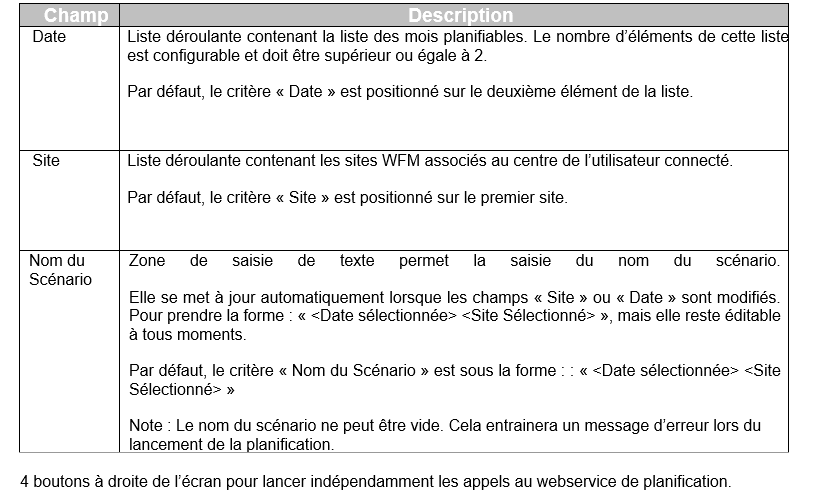
\includegraphics[width=.95\textwidth]{fig/fig18_PlanoHDSIFonct.png}
\insererfigure{fig/fig16_PlanoHDSI.png}{7cm}{Planification Horaire pour utilisateur DSI}{PlanoHDSI}

Tandis que l'UGS est beaucoup plus limité:\\
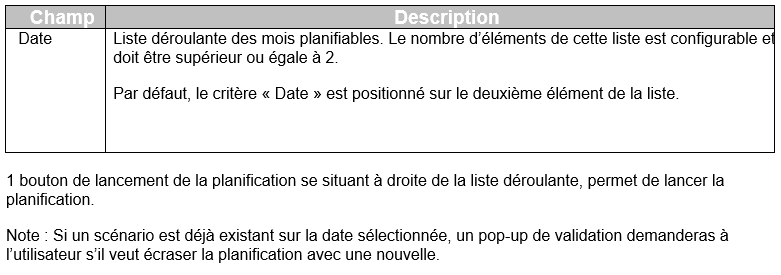
\includegraphics[width=.95\textwidth]{fig/fig19_PlanoHUGSFonct.png}
\insererfigure{fig/fig17_PlanoHUGS.png}{7cm}{Planification Horaire pour utilisateur UGS}{PlanHoUGS}

Cette phase a été pour moi l'occasion, tout en continuant d'en apprendre plus sur le langage et le framework, de tester mes nouvelles connaissances.\\
Elle m'a aussi permis de découvrir de façon concrète l'architecture et les dogmes de l'application OCEAN, ainsi que la librairie Kendo de telerik, utilisée ici pour les composants d'interface Homme Machine (IHM).\\

\subsubsection{Industrialisation du WebService WFM}

Dès lors que nous avons reçu les sources du webservice, nous avons pu constater les soucis qui allaient nous être posé. Résultat d'une année entière de développement par des personnes qui ne sont pas développeurs, il s'agissait d'un unique fichier C\# de sept mille lignes, mélangeant paramètres, données, logique métier, WebMethods ou encore classes d'objets. Le tout avec des fonctions pouvant aller jusqu'au millier de lignes, des signatures de plus de vingt paramètres, des cascades de conditionnelles imbriquées et aucune documentation.\\

\insererfigure{fig/fig20_WFMWebSvcExemple.png}{2cm}{Exemple d'une signature de fonction originelle}{WebSvcEx}

Ce webservice tombant sous la responsabilité de Capgemini, une fois intégré au projet OCEAN, il était primordiale de reprendre ce dernier pour le rendre industrialisable. Et cela en prévision, notamment, de futures évolutions sur ce service, ainsi que de la maintenance de ce dernier.\\

Lors de cette étape, j'ai donc fait en premier lieu de la rétro-ingénierie, afin d'essayer de comprendre la trame globale des appels. Aidé de SonarQube, cela m'a permis de parcourir tout le webservice en corrigeant les nombreux codes smells trouvés par cet outil, tout comme découvrir de possibles bugs.\\
Ensuite accompagné de Mohammed HAMMAMI et en partageant en deux les tâches, nous avons rédigé la documentation hautement nécessaire du webservice, préparant au découpage en fonctions avec une logique minimale.\\

Cette période de mon stage, bien qu'exténuante, m'a entraîné dans la reprise de codes inconnus, exercice que je considère encore à ce jour comme compliqué mais primordial.

\subsubsection{Intégration WFM}

Une fois la documentation et le nettoyage d'une majorité des codes smells faite avec Mohammed HAMMAMI, nous nous sommes lancés dans le découpage des quatre méthodes du WebService afin de les intégrer à l'architecture des services OCEAN. 

\begin{minipage}{0.35\textwidth}
\insererfigure{fig/fig12_OceanWebservicesArchi.png}{3cm}{WebServices}{OceanWebservicesArchibis}
\end{minipage}
\begin{minipage}{0.55\textwidth}
Séparé de telle façon que la façade du webservice soit située dans "Service" afin de jouer le rôle d'API. La logique métier dans "Rules", les appels minimaux vers la solution WFM Genesys dans la section "DAL" et "BO" pour les données et paramètres manipulés.
\end{minipage}
\vspace{5mm} %5mm vertical space
\\

Cela a été pour moi l'occasion de pratiquer sur une partie encore quelque peu inconnue de l'application OCEAN, appréhendant l'architecture de cette dernière pour ses services.

\subsubsection{Connections WFM au Front-End}

Une fois le webservice entièrement intégré et fonctionnel, il ne restait plus qu'a connecté les appels à mon Interface Homme Machine (IHM) au travers de la référence du service WFM maintenant créée, tout en s'assurant du bon fonctionnement des requêtes AJAX envoyées par le javascript.\\

Mon code arrivant à sa finalisation, l'heure est venue de le faire réviser par une personne avec davantage d'expérience. Ainsi Mohammed HAMMAMI, architecte d'OCEAN, a pu me donner des points d'amélioration ainsi que divers conseils comme l'utilisation de certains composants existant dans la solution pour améliorer l'expérience utilisateur. Cela a permis quelques améliorations de ma part sur mon interface.\\

Une fois validé par l'équipe, il ne me restait plus qu'à passer ma production sous l'outil StyleCop, afin de respecter les règles de rédaction de code du projet, et rajoutant parfois des commentaires additionnels.\\

\begin{minipage}{0.55\textwidth}
\insererfigure{fig/fig21_PlanHoDiagramm.png}{9cm}{Diagramme de séquence d'une planification horaire}{PlanHoDiagramm}
\end{minipage}
\begin{minipage}{0.35\textwidth}
La fonction "Planification Horaire" désormais développée et le webservice intégré à la solution:\\

Une planification horaire envoyée par un utilisateur UGS de l'application OCEAN se déroule de la façon ci-contre.\\

Quatre appels séquentiels ont lieu vers le webservice WFM contenant la logique pour le paramétrage, au travers d'appels, de la solution WFM Genesys.

\end{minipage}
\vspace{5mm} %5mm vertical space
\\

Finalisant les tâches de développement pour la fonction de planification horaire du module WFM, j'ai reçu des avis sur mon code me permettant d'améliorer l'ergonomie et de ne pas oublier des cas d'utilisation extrême.

\subsubsection{Tests WFM}

Jusqu'ici, afin de s'assurer du bon fonctionnement du webservice, nous nous sommes assuré de la génération de tables de planification dans l'outil WFM de Genesys après que le webservice soit appelé.\\
Il nous fallait cependant tester l'intégrité du webservice une fois optimisé et découpé dans notre solution, afin de s'assurer de son bon fonctionnement. De par la nature possiblement imprévisible de la planification Genesys, il nous était impossible de tester le résultat de cette dernière en comparant tout simplement la planification du webservice originel à la notre.\\

Il s'agissait ici d'un point critique de la reprise du webservice:\\
nous ne pouvions laisser le webservice en l'état à sa réception, mais l'industrialiser risquait d'impacter la logique de ce dernier.\\

Lors de sa production, le webservice était testé à l'aide de tableurs Excel décorés par du Visual Basic, et nourris par les export CSV (Comma-separated values) de la planification générée. Ces tables permettaient notamment de s'assurer du respect des contraintes salariales ou d'activité.\\
Néanmoins, ces tableurs ont vite été abandonnés avec la complexité croissante du webservice, les rendant inutilisables.\\
Une migration a alors été faite vers l'outil SAS Enterprise Guide, qui permet l'analyse complexe de données. Ce dernier a donc été majoritairement utilisé pour tester la planification et leur aurait permis de valider le webservice.\\
Cependant ce dernier fût hors de notre portée, ne possédant pas la connaissance technique du logiciel (même après avoir cherché des connaissances auprès des communautés Capgemini), et n'ayant pas accès à une licence de l'outil (absent des outils accessibles par le groupe).\\

\begin{minipage}{0.35\textwidth}
Il fallait donc trouver une autre solution. Après un brainstorming avec Bastien CLOAREC, nous sommes arrivés à la conclusion que nous pourrions tester la logique en vérifiant les appels envoyés entre le webservice et la solution (comme pointé ci-contre).\\

Il suffirait d'écouter dans les mêmes conditions les quatre messages envoyés par le webservice valide et le webservice à tester, vers la solution.\\
Ensuite il suffit de comparer et d'étudier les différences dans les paquets partagés, afin de s'assurer du fonctionnement.\\
\end{minipage}
\begin{minipage}{0.55\textwidth}
\insererfigure{fig/fig22_PlanHoDiagrammTests.png}{9cm}{Diagramme de séquence d'une planification horaire}{PlanHoDiagrammTest}
\end{minipage}
\vspace{5mm} %5mm vertical space
\\

Je me suis donc attelé à la mise en place du protocole pour ce test:\\
A l'aide de WireShark, j'ai donc pu extraire les paquets échangés entre ces deux éléments puis j'ai pu développer en Batch Windows un script pour ranger et supprimer le surplus d'informationdans des fichiers séparés. Initialement, je voulais le faire en python pour la simplicité, mais ne voulant pas alourdir l'environnement de développement déjà imposant, je me suis orienté vers une technologie que tout le monde avait déjà sur son poste. \\


Cette technique, bien que rébarbative, m'a permis après les premiers passages de déceler quelques erreurs d'inattentions lors du découpage du webservice, pouvant entraîner notamment différents effets de bords indésirables pour la planification.\\

Cette étape m'a permis de refaire un passage sur l'intégration de ce nouveau service, entraînant la résolution de différents bugs. J'ai aussi passé du temps pour rédiger les tests fonctionnels de ma fonction OCEAN, en vue de la livraison qui approche, dans l'outil HP Application Lifecycle Management (HP AML) en expliquant notamment en détail le déroulement des tests du webservice.\\

Ce sera plus tard cependant, après un échange avec un ingénieur spécialisé dans les plate-formes de tests, que j'ai découvert l'existence de Mock Server qui aurait pu simplifier grandement notre technique de test.

\subsubsection{Documentation WFM}

Ici, je me suis plongé dans la rédaction de la documentation pour mes actions sur OCEAN, et en  parallèle, l'équipe passait mes tests en prévision de la livraison de l'évolution.\\

J'ai ainsi mis à jour les documentations exhaustives suivantes:
    \begin{itemize}
        \item Documentation d'Administration Fonctionnelle SFDU, pour expliquer le comportement de l'application à un utilisateur
        \item Documentation d'Administration Technique SFDI, pour expliquer la technique de l'application.
        \item Document d'exploitation MEX, pour les paramétrages et configurations possibles de l'outil, à destination des techniciens installant l'application chez le client.
    \end{itemize}

Au terme de cette période, l'évolution fût envoyée chez le client, terminant cette tâche générale pour le projet.

\newpage
\subsection{Évolution des Documents dans les AcTions pour le Bandeau}

Dans le bandeau, deux types d' AcTions existent dans la bannette d'un utilisateur: on y retrouve les e-mails et les tâches.\\
Avant cette évolution, seul les e-mails pouvaient posséder des documents joints sous la forme suivante:

\insererfigure{fig/fig23_PJEmail.png}{5cm}{Modèle de consultation d'un email}{PJEmails}

L'idée de cette évolution est de rajouter dans les tâches un composant semblable pour rajouter des pièces jointes à une tâche. Cela implique par ailleurs l'intégration des manipulations d'une pièce jointe, ainsi que sa récupération.\\

\subsubsection{Composant pièce jointe dans les Tâches}

Bastien CLOAREC s'occupait de modifier le service iWD (un sous-système permettant notamment la création de tâches) afin qu'il supporte des documents joints. Je me suis mis en renfort sur cette évolution afin de rajouter un nouveau composant pour les tâches, permettant d'afficher ces pièces jointes.\\

Une tâche sur le bandeau est modélisée comme un formulaire que l'opérateur remplit. Cependant, chaque tâche est différente et répond à des problématiques métiers différentes. C'est pourquoi leur interface est hautement configurable au sein du Configuration Manager (CME), où il est possible de créer une interface entièrement personnalisée pour une nouvelle tâche, en déclarant pour chaque ligne quels composant ont y retrouve et sa localisation.

\insererfigure{fig/fig24_IHMTache.png}{6cm}{Configuration de la première ligne d'une tâche de déclaration d'Iphone}{IHMTache}

Pour créer ce nouveau composant, il me suffit de me référer à celui déjà existant sur les e-mails, en m'assurant qu'il soit autonome pour être intégré aux composants disponibles pour les tâches.\\
Cependant, ce composant utilise une classe "EmailInteraction", foncièrement différente à la nouvelle classe "TaskInteraction", et qui est nécessaire pour la logique des classes fonctionnelles.\\
Il fut alors pris la décision de créer une interface pour les deux composants, afin que les classes fonctionnelles puissent être réutilisées dans les deux types composants, sans duplication de code. \\

\insererfigure{fig/fig25_EvolutionArchi.png}{6cm}{Comparaison de l'architecture des Interaction avant et après l'évolution}{EvolutionBMArchi}

Cela m'a permis de toucher pour une toute première fois au code du Bandeau, ne découvrant qu'une petite partie de ce dernier, en modifiant cependant beaucoup de classes. Mais au terme de cette évolution, une fois que Bastien CLOAREC a eu fini avec les services pour supporter les pièces jointes, nous avons pu livrer au client (après une mise à jour des documentation et une période de tests).\\

\insererfigure{fig/fig26_DocumentComponent.png}{1cm}{Composant pièces jointes des tâches}{DocumentComponent}


\subsubsection{Amélioration pièce jointe dans les Tâches}

Plus d'un mois après la livraison de l'évolution offrant la possibilité à un opérateur de consulter des pièces jointes pour une tâche, une nouvelle expression de besoin arriva. Il s'agissait d'une amélioration du composant de pièces jointes, afin d'informer l'utilisateur de la mauvaise réception de document(s), et lui permettre de tenter la récupération de ce(s) dernier(s).\\

En effet, avant d'être associés à une tâche, les documents qui leurs sont destinés doivent dans un premier temps passer par un service de catégorisation des fichiers (propre au client, notre projet ni ayant pas accès). Seul souci, il arrive que ce service tombe, empêchant le traitement de ces documents et donc l'affiliation à une tâche.\\

Ainsi, le nouveau composant des pièces jointes se devait à la fois d'informer du manque de documents pour l'agent, mais aussi offrir une possibilité de relancer la catégorisation afin de récupérer les pièces.\\

\insererfigure{fig/fig27_DocumentComponentError.png}{0.5cm}{Composant pièces jointes des tâches avec erreurs}{DocumentComponentError}

Cette amélioration a demandé une retouche des services, de Bastien CLOAREC, pour informer le Front-End, tandis que j'appliquais les modifications sur mon Interface Homme Machine (IHM).\\

Après une seconde mise à jour des documentations et une période de tests, cette évolution fût livrée.\\

\newpage
\subsection{Autres}
Je vais ici parler des petites actions réalisées, ne méritant pas une partie à elles toutes seules.\\
Ainsi, je vais parler de diverses livraisons et périodes de tests dans lesquelles j'étais impliqué; de quelques corrections d'anomalies sur lesquelles j'ai joué un rôle; l'expression de besoins pour laquelle j'ai participé à l'estimation du chiffrage des actions; une étude sur l'environnement jenkins déjà en place; et enfin les différentes formations que j'ai pu assister lors de mon stage.

\subsubsection{Livraisons}

Une fois une évolution développée, cette dernière va en recette en prévision de la livraison. Cette étape consiste à tester l'application par une tierce personne n'ayant, possiblement, pas développé la partie impactée.\\
Étant une petite équipe, mais travaillant en parallèle sur plusieurs évolutions, il arriva de nombreuses fois à participer à la livraison en passant des tests.\\

Les deux premières livraisons auxquelles j'ai participé ont été l'occasion pour le projet de passer des tests de non régressions. Ces derniers ont permis de refaire un passage sur la majorité des fonctionnalités de chacune des applications, découvrant parfois quelques bugs. \\
Elles m'ont permis par la même occassion de me familiariser avec l'environnement découvrant en détail le Bandeau et OCEAN, ainsi que le fonctionnement de la configuration genesys.

\subsubsection{Correction d'anomalies}

Les bugs sont un élément courant dans la vie de développeur. Lorsque le projet livre une nouvelle amélioration, cette dernière passe du côté client une batterie de test avant d'être envoyée en production.\\

Lors de ces étapes, le client peut ainsi découvrir des anomalies qu'il nous fait remonter au travers d'HP ALM (HP Application Lifecycle Management). Dès lors, l'équipe doit répondre à ces dernières (sous garantie ou non), offrant une solution pour la résolution de cette dernière.\\

Tout le long de mon stage, des anomalies ont pu être signalées par le client. Il s'agissait parfois de simples soucis de configuration, mais chaque bug m'a permis d'aller fouiller dans différents coins de l'application, m'entraînant à la relecture de code et documentations, pour identifier les problèmes.

\subsubsection{Étude d'expression de besoins}

En fin de stage, après un creux d'activité, une expression de besoins imposante a fait son arrivée. Pour accélérer son étude, Bastien CLOAREC m'a offert la possibilité de l'assister sur certains points d'évolution. Étant familiarisé avec l'application OCEAN, j'ai donc réalisé un chiffrage pour le développement de ces évolutions pour l'application.

\subsubsection{Étude environnement Jenkins}

L'outil Jenkins est utilisé notamment pour générer des builds journaliers, passant des tests et générant un rapport de couverture de tests OpenCover.\\
Pour un soucis de centralisation de reporting, SonarQube a été installé pour ses rapports de qualité de code.\\
Il m'a été demandé de passer à sonar le rapport OpenCover. Malgré un échec lié à une version non supportée des rapports par SonarQube, ce fut pour moi une première introduction à l'outil Jenkins, et son fonctionnement.

\subsubsection{Formations}

Lors de notre stage, de nombreuses formations ont pris place majoritairement dans le but de nous faire découvrir les communautés et leurs différents acteurs. Ces formations surtout techniques étaient une preuve d'implication de l'entreprise dans le partage des connaissances.\\

Parmi elles, on peut compter:
\begin{itemize}
    \item Formation "DevOPS"
    \item Formation "Méthodes Agile, Scrum, Safe"
    \item Formation "Gestion de la configuration"
    \item Formation "Architecture logiciel et construction d’une solution WEB"
    \item Formation "Tests unitaires et BDD"
    \item Formation "Intégration / Performance / Sécurité"
\end{itemize}


\newpage
%-----------------BILAN -----------------------------
\section{Bilan}

Le but de mon stage était de découvrir à la fois le monde de l'entreprise, ainsi que de nouvelles technologies, et je dois dire que je ne suis pas déçu, à la fois professionnellement que personnellement!\\

J'ai pu intégrer une véritable équipe de développement, participer à la vie du projet, répondant à des problématiques diverseq. J'ai pu faire de l'étude de besoin, jusqu'à de la livraison de solutions, tout en passant par du développement, des tests, de la rédaction de documentations et de la maintenance de l'existant. Ce stage m'a permis d'acquérir des connaissances primordiales dans la production industrielle de solutions numériques.

Ce projet m'a permis de découvrir une partie du framework .NET et de son environnement, une technologie qui reste aujourd'hui grandement utilisée dans le monde professionnel.
Mes travaux ont pu être critiqués par des professionnels, me permettant d'appréhender les défauts dans mes choix d'implémentation avant de les corriger. \\

Personnellement, l'expérience a été enrichissante. Des points d'amélioration m'ont été soumis pour mon avenir, et la pratique du métier m'a conforté dans mes choix.

\section*{Summary}

The end goal of my internship was to both discover new technologies and corporate world. And I'll have to admit, I wasn't let down, both professionally and personally!\\

I've been able to take part in a legitimate team of developers. Getting involved in the life cycle of a project, answering diverse issues. Going from needs analysis to delivery, working through development, testing, updating documentation, and maintaining existing solutions. This internship granted me mandatory knowledge on the industrial production of digital solutions.\\

This project allowed me to discover a part of the .NET framework and environment. Something that, to this day, is still relevant in the industry.
My work was able to be reviewed and criticized by professionals, allowing myself to figure out issues with my choices, before correcting them.\\

Personally, this was a rewarding experience. Some key  improvement was shared with me for my future, and the practice of the profession reassured me.

\subsection*{Conclusion}
Pour résumer, arrivant au terme de mon stage, le bilan me parait très satisfaisant. \\
Apprendre de nouvelles technologies était pour moi un point central de ce stage, et j'ai eu le droit à bien plus que ça. J'ai fait mon maximum pour répondre aux demandes de l'équipe, et je ressens une certaine satisfaction pour mes travaux réalisés. \\
J'en ressors avec des réponses et des connaissances pour mon avenir, mais aussi avec une proposition de contrat à durée indéterminée.

\end{document}
